\begin{question}
\noindent $A$, $B$ and $C$ are points on the circumference of a circle with centre $O$.

\noindent Find the size of angle $ACB$, marked $x$ on the diagram.

\begin{center}
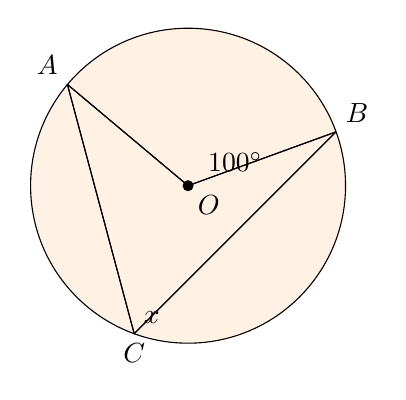
\begin{tikzpicture}[scale=2]
    \coordinate (O) at (0,0);
    \coordinate (A) at (140:1);
    \coordinate (B) at (20:1);
    \coordinate (C) at (250:1);

    \draw[fill = orange!10] (0,0) circle (1);
    \fill[black] (0,0) circle (1pt);

    \draw (O) -- (A);
    \draw (O) -- (B);
    \draw (A) -- (C);
    \draw (C) -- (B);

    \node[above left] at (A) {$A$};
    \node[above right] at (B) {$B$};
    \node[below] at (C) {$C$};
    \node[below right] at (O) {$O$};

    \draw (A) -- (O) -- (B);
    \node at (0.3, 0.15) {$100^\circ$};
    
    \draw (B) -- (C) -- (A);
    \node at (C) [above right] {$x$};
\end{tikzpicture}
\end{center}

\vspace{4cm}
\begin{flushright}
    \answerequnit{x}{$^\circ$}{2}
\end{flushright}
\end{question}